\documentclass[uplatex,dvipdfmx,a4paper,11pt]{jsarticle}

\usepackage{url}
\usepackage[dvipdfmx]{hyperref}

\usepackage[top=25mm,bottom=25mm,left=25mm,right=25mm]{geometry}

\usepackage{array}
\usepackage{tabularx}
\usepackage{booktabs}
\usepackage{enumitem}
\usepackage{graphicx}
\usepackage{longtable}
\usepackage{listings}

\lstset{
  basicstyle=\ttfamily\scriptsize,
  breaklines=true,
  frame=single,
  numbers=left,
  numberstyle=\tiny,
  tabsize=2,
  showstringspaces=false
}

\setlength{\parindent}{0pt}
\setlength{\parskip}{0.6em}

\usepackage{titlesec}
\titleformat{\section}
  {\normalfont\Large\bfseries}{\thesection.}{0.6em}{}
\titleformat{\subsection}
  {\normalfont\large\bfseries}{\thesubsection}{0.6em}{}
\titlespacing*{\section}{0pt}{1.2em}{0.6em}
\titlespacing*{\subsection}{0pt}{1.0em}{0.4em}

\newcommand{\sectionrule}{\par\medskip\noindent\rule{\linewidth}{0.6pt}\par\medskip}

\renewcommand{\labelitemi}{\textbullet}
\renewcommand{\labelitemii}{\textopenbullet}
\setlist[itemize]{leftmargin=1.6em,itemsep=0.1em,topsep=0.2em}
\setlist[enumerate]{leftmargin=2.0em,itemsep=0.1em,topsep=0.2em}

\providecommand{\textopenbullet}{\ensuremath{\circ}}


\begin{document}


{\LARGE\bfseries 作業ログ}\par\bigskip

報告者：佐藤涼菜

報告日：6月23日

プロジェクト名：マジカル☆観覧車

\sectionrule


\section{進捗サマリー（要約）}

\begin{itemize}
  \item 全体進捗率：85[％]
  \item マイルストーン達成状況：おおよそ達成（テストフェーズは結合待ち）
  \item 主要成果：
    \begin{itemize}
      \item {指揮デバイスの最終固定および加工をし，本体・センサの実装（No.2112）を完了}
      \item {BPM・音量変化機構の実装（No.2113）を完了}
      \item {計画書との変更点の記述（No.2231）}
    \end{itemize}
  \item 重大課題（影響度：高）：
    \begin{itemize}
      \item {テストフェーズ（No.3241）が結合待ちのため未着手}
    \end{itemize}
\end{itemize}

\sectionrule


\section{作業ログ（詳細トラッキング）}

\subsection{作業ログ}

\renewcommand{\arraystretch}{1.2}

\small

\begin{longtable}{|c|p{2.2cm}|c|c|c|c|p{2.4cm}|p{3.1cm}|}
\caption{作業ログ} \\
\hline
No. & 作業項目 & 開始日 & 予定完了日 & 状態 & 進捗率 & 依存関係・ブロッカー & コメント \\
\hline
\endfirsthead

\hline
No. & 作業項目 & 開始日 & 予定完了日 & 状態 & 進捗率 & 依存関係・ブロッカー & コメント \\
\hline
\endhead

\hline
\multicolumn{8}{r}{次ページへ続く} \\
\hline
\endfoot

\hline
\endlastfoot

2112 &
本体・センサの実装 &
5/24 &
6/17 &
完了 &
100\% &
無 &
回路の最終固定と筐体の加工を行った．\\
\hline



2113 &
BPM・音量変化機構の実装 &
5/29 &
6/1 &
完了 &
100\% &
無 &
スライド式可変抵抗器の動作確認を実施し完了．\\
\hline

3241 &
LEDマトリクスの反映確認 &
6/17 &
6/30 &
未着手 &
0\% &
有 & 
結合テストの実施待ち．6/24の授業内にて実施予定．\\
\hline

- &
作業ログの記入 &
6/17 &
6/23 &
完了 &
100\% &
無 &
特になし．\\
\hline



\end{longtable}


\subsection{日ごとの作業ログ}


    \renewcommand{\arraystretch}{1.2}

    \small

    \begin{longtable}{|c|c|p{2.4cm}|c|c|c|c|p{3.8cm}|}
    \caption{日ごとの作業ログ} \\
    \hline
    日付 & No. & 作業項目 & 時間 & 開始時の状態 & 終了時の状態 & 進捗率 & コメント \\
    \hline
    \endfirsthead

    \hline
    日付 & No. & 作業項目 & 時間 & 開始時の状態 & 終了時の状態 & 進捗率 & コメント \\
    \hline
    \endhead

    \hline
    \multicolumn{8}{r}{次ページへ続く} \\
    \hline
    \endfoot

    \hline
    \endlastfoot

    6/17 & 2113 & BPM・音量変化機構の実装 & 1.5h &
    おおよそ完了 &
    完了 &
    100\% &
    スライド式可変抵抗器の再はんだ付けおよび動作確認を実施し完了．\\
    \hline

    6/18 & 2112 & 本体・センサの実装 & 1h &
    進行中 &
    進行中 &
    93\% &
    内部配線の整理と筐体を加工するための備品調達．\\
    \hline

    6/19 & 2112 & 本体・センサの実装 & 2h &
    進行中 &
    進行中 &
    96\% &
    操作部の露出加工．筐体の加工．\\
    \hline

    6/20 & 2112 & 本体・センサの実装 & 1.5h &
    進行中 &
    進行中 &
    98\% &
    回路の最終固定と筐体内部の配線固定を実施．\\
    \hline

    6/21 & 2112 & 本体・センサの実装 & 0.5h &
    進行中 &
    完了 &
    100\% &
    筐体の最終仕上げを行い，本体・センサの実装を完了．\\
    \hline

    6/22 & 2231 & LEDマトリクス制御 & 1h &
    完了 &
    完了 &
    100\% &
    計画書と実装の変更点を整理し記述．\\
    \hline

    6/23 & - & 作業ログの記入 & 1h &
    未着手 &
    完了 &
    100\% &
    特になし．\\

    \end{longtable}

\sectionrule

\section{計画時のGCと現在のGC}

計画段階のガントチャート(GC)を図\ref{fig:gant7}（実装フェーズ）および図\ref{fig:gant8}（テストフェーズ）に示す．

\begin{figure}[htbp]
    \centering
    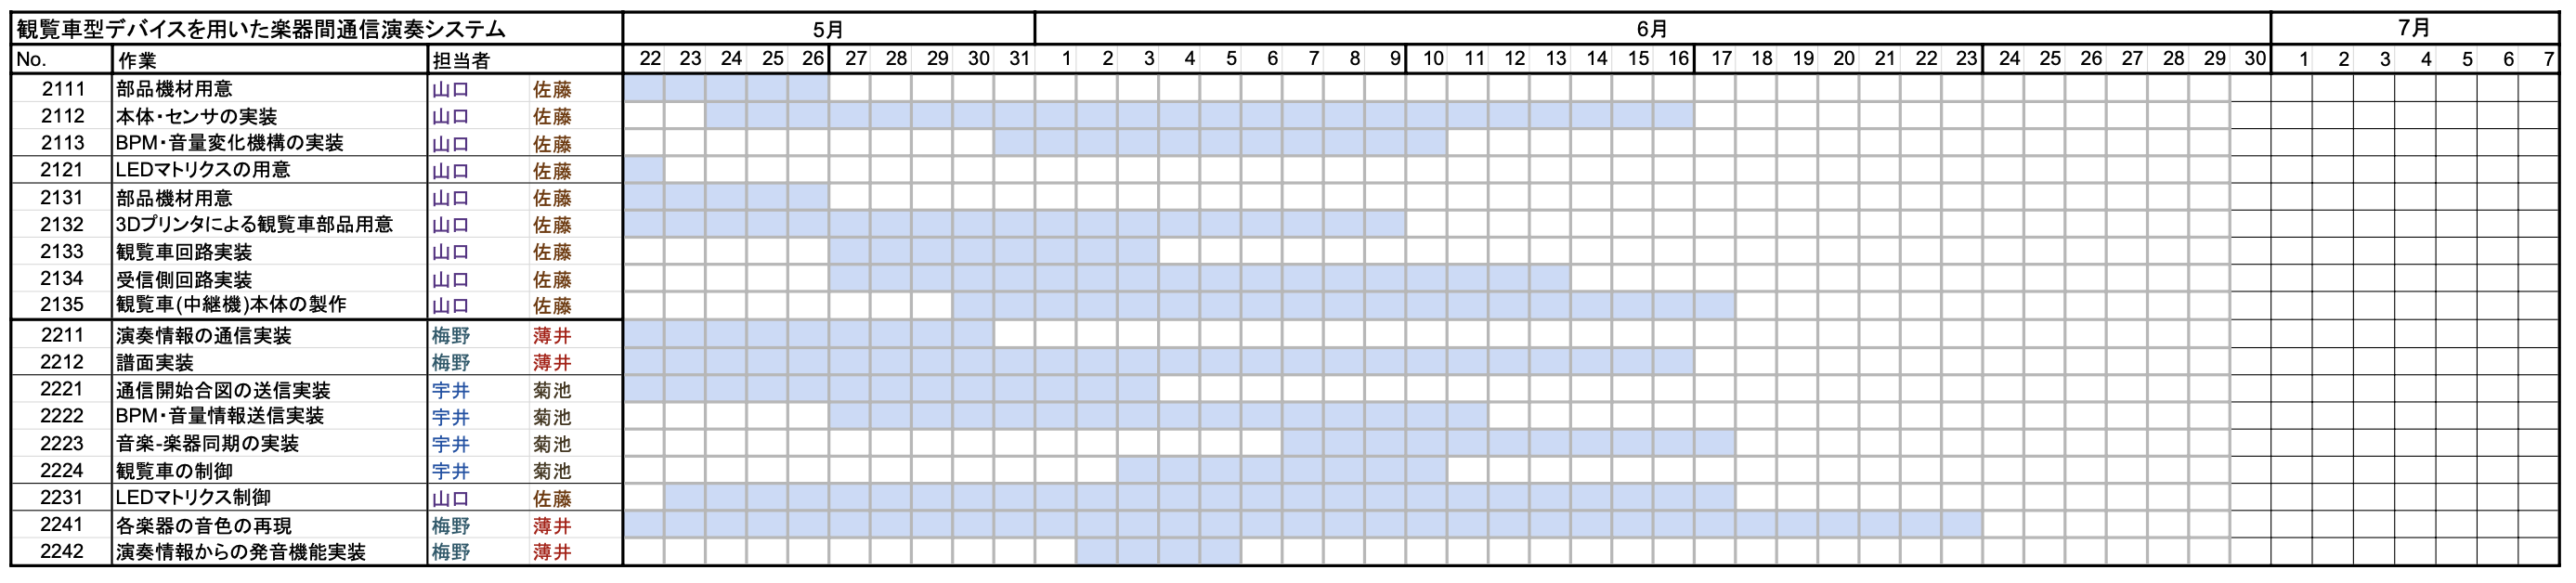
\includegraphics[width=0.9\columnwidth]{gant7.png}
    \caption{計画段階のガントチャート（実装フェーズ）}
    \label{fig:gant7}
\end{figure}

\begin{figure}[htbp]
    \centering
    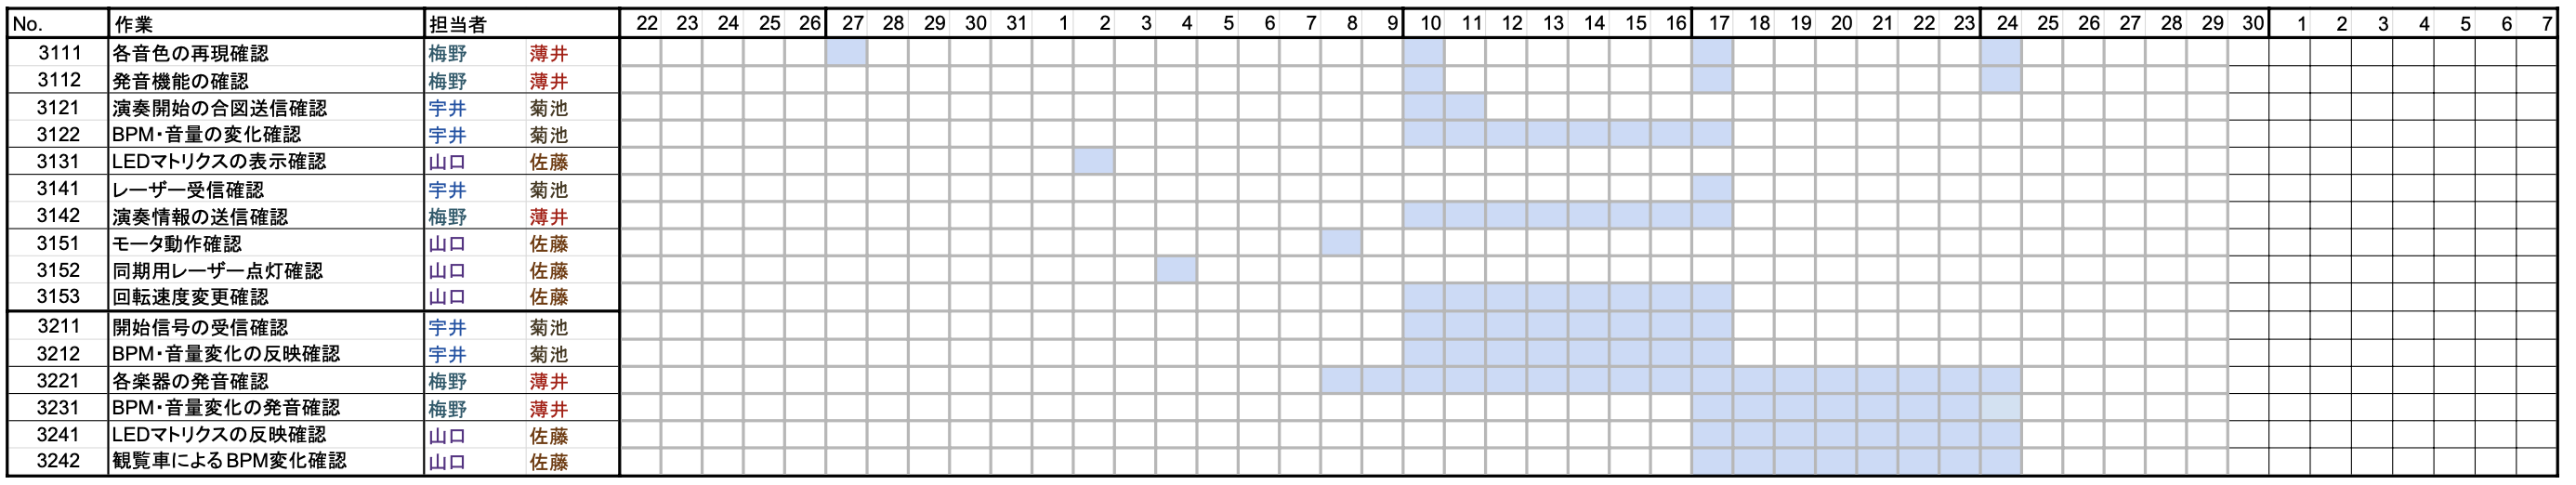
\includegraphics[width=0.9\columnwidth]{gant8.png}
    \caption{計画段階のガントチャート（テストフェーズ）}
    \label{fig:gant8}
\end{figure}

次に，現在のGCを図\ref{fig:gant10}に示す．達成した項目は緑色で塗られている．

\begin{figure}[htbp]
    \centering
    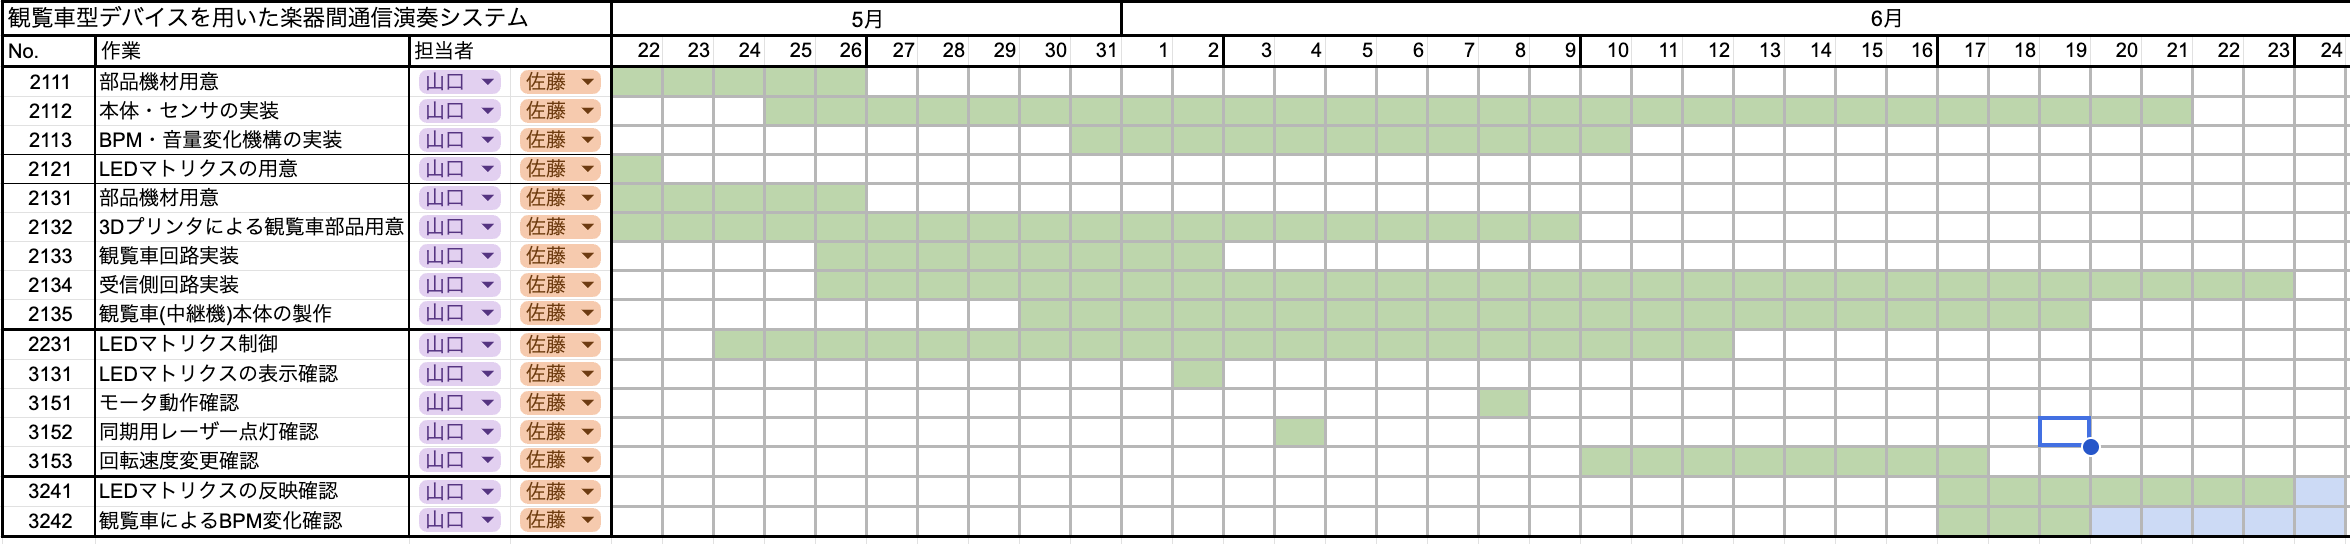
\includegraphics[width=0.9\columnwidth]{gant10.png}
    \caption{現在のガントチャート}
    \label{fig:gant10}
\end{figure}


\sectionrule


\section{課題管理}

\begin{tabularx}{\linewidth}{@{}p{3cm}Xllp{3.2cm}ll@{}}
\toprule
課題 & 発生原因 & 影響度 & 優先度 & 対策 & 期限 & 状態 \\
\midrule
可変抵抗器がブレッドボード上で安定接続できない（No.2112/2113に影響） & スライド式可変抵抗器の端子形状がブレッドボードに適合しないため． & 高 & 高 & スライド式可変抵抗器を基盤に設置し，筐体へ固定した． & 6/12 & 対応済 \\
\midrule
1機のスライド式可変抵抗器のはんだ付け設置不良（No.2112に影響） & 基盤へのはんだ付け時に接触不良が発生したため． & 中 & 高 & 6/17に再はんだ付けを実施し，動作を確認した． & 6/17 & 対応済 \\
\midrule
テストフェーズが結合待ち（No.3241に影響） & 通信系との結合が完了していないため，LEDマトリクスの反映確認テストが実施できない． & 高 & 中 & 通信系の準備完了を待ち，結合テストを実施する． & 6/30 & 対応中 \\
\bottomrule
\end{tabularx}

\medskip
※影響度＝プロジェクトへのインパクト

※優先度＝対応の緊急性

\sectionrule


\section{AI利用状況と検証（再現性重視）}

今回はAIを利用していない．

\sectionrule


\section{No.2231 LEDマトリクス制御：計画書との変更点}

\subsection{描画APIの変更}

計画書（3.5.8.3）では，フレームバッファの描画に
\texttt{matrix.renderBitmap()}を使用すると記述されている．
\texttt{renderBitmap()}は\texttt{uint8\_t[8][12]}形式の配列を引数に取る関数である．
実装では\texttt{uint32\_t[3]}形式にビットパックし，
\texttt{matrix.loadFrame()}で描画する方式に変更した．
これは，\texttt{loadFrame()}の方がフレームバッファのメモリ効率が高く，
96ビット（8行$\times$12列）を3つの32ビット整数で表現できるためである．

\subsection{関数の追加}

計画書の表3.33には\texttt{checkUDP}と\texttt{displayBPM}の2関数のみ記載されている．
実装では以下の3関数を追加した．

\begin{itemize}
  \item \texttt{clearDisplay()}: 演奏終了ヘッダ（'E'）受信時にLEDマトリクスを全消灯する関数．
  計画書の通信プロトコル（表3.29, 3.30）にはヘッダ'E'が定義されているが，
  Display側の関数一覧にはこの処理への言及がなかったため追加した．

  \item \texttt{drawDigit()}: 1桁の数字を独自フォント（\texttt{font3x5[]}）を参照して
  フレームバッファに描画する内部関数．
  \texttt{displayBPM()}から桁ごとに呼び出される．

  \item \texttt{displaySetup()}: \texttt{matrix.begin()}をDisplay.cpp側で呼ぶための
  初期化関数．\texttt{Arduino\_LED\_Matrix}の表示バッファはヘッダ内でstatic定義されており，
  includeする翻訳単位ごとに別実体となる．そのため，描画を行う\texttt{loadFrame()}と
  同一ファイルから\texttt{begin()}を呼び出す必要があり，本関数を追加した．
\end{itemize}

\subsection{モジュール構成の変更}

計画書の図3.16では\texttt{checkUDP()}はDisplay.ino側に配置されている．
実装ではDisplay.cppに移動した．
\texttt{checkUDP()}内で\texttt{currentBPM}（Display.cppの静的変数）を参照する必要があるためである．
これにより，Display.inoには\texttt{setup()}と\texttt{loop()}のみが残る構成となった．

\subsection{受信データの読み込み形式}

計画書（3.5.8.3）では「ペイロードを文字列として読み込む」と記述されている．
実装では\texttt{uint8\_t buffer[2]}としてバイナリ形式で読み取り，
\texttt{buffer[0]}をヘッダ文字（char），\texttt{buffer[1]}を段階番号（uint8\_t）として処理している．
通信プロトコル仕様（表3.29, 3.30）自体は固定長2バイトのバイナリ形式で定義されており，
実装側がプロトコル仕様に忠実な形式を採用した．

\subsection{静的IP設定の追加}

計画書の表3.24にはDisplay側の定数として\texttt{localIP}（観覧車デバイス自身の静的IPアドレス）が
定義されている．実装では\texttt{WiFi.config(localIP, gateway, subnet)}を
\texttt{WiFi.begin()}の前に呼び出すことで，
指揮デバイスの送信先IPアドレス（192.168.11.10）と一致する固定IPを設定した．

\sectionrule


\section{次回計画}


\begin{itemize}

  \item 目標：通信系との結合テストの実施
    \begin{itemize}
      \item 通信系の準備が完了次第，
      LEDマトリクスの反映確認テスト（No.3241）を実施する．

      \item 指揮デバイスからのUDP送信によりBPM値がLEDマトリクスに
      正しく表示されることを確認する．
    \end{itemize}

  \item 達成基準：
    \begin{itemize}
      \item 指揮デバイスからBPM値を送信し，
      表示デバイスのLEDマトリクスに正しく反映されること．

      \item 演奏終了ヘッダ（'E'）の受信時にLEDマトリクスが消灯すること．
    \end{itemize}

  \item 期限：
    \begin{itemize}
      \item 2026/6/30
    \end{itemize}

\end{itemize}


\sectionrule


\section{付録}

No.2231（LEDマトリクス制御）のプログラムを以下に示す．

\subsection{Display.h}
\begin{lstlisting}
#ifndef DISPLAY_H
#define DISPLAY_H

#include <Arduino.h>
#include "Arduino_LED_Matrix.h"  // Arduino UNO R4 WiFi 内蔵LEDマトリクス用ライブラリ
#include <WiFiS3.h> //UDP通信

// BPM定数定義
#define BPM_STEP_1  60
#define BPM_STEP_2  90
#define BPM_STEP_3  120
#define BPM_STEP_4  150
#define BPM_STEP_5  180

// 通信定数
#define LOCAL_PORT     2390   // UDP受信に利用するポート番号
#define HEADER_BPM     'B'    // BPMデータ受信の識別ヘッダ
#define HEADER_END     'E'    // 演奏終了の識別ヘッダ（LEDマトリクス消灯）

// 文字フォントの寸法
#define FONT_WIDTH   3   // 1文字の横ドット数
#define FONT_HEIGHT  5   // 1文字の縦ドット数

// LEDマトリクスの寸法（Arduino UNO R4 WiFi 内蔵：8行×12列）
#define MATRIX_ROWS  8
#define MATRIX_COLS  12

// 関数宣言

// LEDマトリクスの初期化（matrix.begin()を本関数経由で呼ぶ。
void displaySetup();

// 中継機からのUDPパケット確認，BPM値の受信処理
void checkUDP();

// 受信したBPM値をLEDマトリクスに数値表示する（引数：int bpm）
void displayBPM(int bpm);

// LEDマトリクスを全消灯する（演奏終了時に使用）
void clearDisplay();

// 指定された1桁の数字を，共有フレームバッファの x_offset 列から描画する
void drawDigit(int digit, int x_offset);

// 外部参照

// 3×5（横3×縦5）の独自数字フォント（0〜9）
extern const uint8_t font3x5[10][15];

// LEDマトリクスインスタンス（Display.cpp で定義，.ino の setup() で begin() を呼ぶ）
extern ArduinoLEDMatrix matrix;

// UDP通信オブジェクト
extern WiFiUDP Udp;

#endif
\end{lstlisting}

\subsection{Display.ino}
\begin{lstlisting}
#include "Display.h"

WiFiUDP Udp;

const char SSID[] = "hackathon001-WPA2";
const char PASS[] = "hackathon001";

// 静的IP設定（指揮デバイスの送信先 ferrisWheelIP2 と一致）
IPAddress localIP(192, 168, 11, 10);
IPAddress gateway(192, 168, 11, 1);
IPAddress subnet(255, 255, 255, 0);

void setup() {
  displaySetup();

  if (SSID[0] != '\0') {
    WiFi.config(localIP, gateway, subnet);
    while (WiFi.begin(SSID, PASS) != WL_CONNECTED) {
      delay(1000);
    }
  }
  Udp.begin(LOCAL_PORT);
}

void loop() {
  checkUDP();
}
\end{lstlisting}

\subsection{Display.cpp}
\begin{lstlisting}
#include "Display.h"
#include "Arduino_LED_Matrix.h"

// 独自フォント定義
// font3x5[digit][row*FONT_WIDTH + col] : 1=点灯, 0=消灯

const uint8_t font3x5[10][15] = {
  // 0
  {1, 1, 1,
   1, 0, 1,
   1, 0, 1,
   1, 0, 1,
   1, 1, 1},
  // 1
  {0, 1, 0,
   1, 1, 0,
   0, 1, 0,
   0, 1, 0,
   1, 1, 1},
  // 2
  {1, 1, 1,
   0, 0, 1,
   1, 1, 1,
   1, 0, 0,
   1, 1, 1},
  // 3
  {1, 1, 1,
   0, 0, 1,
   0, 1, 1,
   0, 0, 1,
   1, 1, 1},
  // 4
  {1, 0, 1,
   1, 0, 1,
   1, 1, 1,
   0, 0, 1,
   0, 0, 1},
  // 5
  {1, 1, 1,
   1, 0, 0,
   1, 1, 1,
   0, 0, 1,
   1, 1, 1},
  // 6
  {1, 1, 1,
   1, 0, 0,
   1, 1, 1,
   1, 0, 1,
   1, 1, 1},
  // 7
  {1, 1, 1,
   0, 0, 1,
   0, 0, 1,
   0, 0, 1,
   0, 0, 1},
  // 8
  {1, 1, 1,
   1, 0, 1,
   1, 1, 1,
   1, 0, 1,
   1, 1, 1},
  // 9
  {1, 1, 1,
   1, 0, 1,
   1, 1, 1,
   0, 0, 1,
   1, 1, 1}
};

// bpmTable[stage-1] で対応するBPMを得る
static const int bpmTable[5] = {
  BPM_STEP_1,  //  60
  BPM_STEP_2,  //  90
  BPM_STEP_3,  //  120
  BPM_STEP_4,  //  150
  BPM_STEP_5   //  180
};

// LEDマトリクスのインスタンス（8行×12列）
ArduinoLEDMatrix matrix;

// displaySetup（LEDマトリクスの初期化）
// Arduino_LED_Matrix の表示バッファ(framebuffer)はヘッダ内で static 定義
// されており，include する翻訳単位(.ino / .cpp)ごとに別実体となる．そのため
// 表示を駆動する割り込みを登録する begin() と，描画を行う loadFrame() は
// 必ず同一ファイル(本 Display.cpp)から呼び出し，同じ framebuffer を共有させる．
// .ino からは matrix を直接触らず，本関数と displayBPM() を呼ぶ

void displaySetup() {
  matrix.begin();

  // begin() 直後の最初の loadFrame は反映されない場合があるため，
  // 消灯フレームを一度描画(ウォームアップ)してから安定するまで待機する．
  uint32_t warmUp[3] = {0, 0, 0};
  matrix.loadFrame(warmUp);
  delay(200);
}

// 描画用共有フレームバッファ（MATRIX_ROWS行 × MATRIX_COLS列，1=点灯 / 0=消灯）
// drawDigit() がここに書き込み，displayBPM() がまとめてレンダリングする
static uint8_t frameBuffer[MATRIX_ROWS][MATRIX_COLS];

// 直近に表示中のBPM値（更新検知用：値が変化した時だけ再描画する）
static int currentBPM = -1;

// checkUDP
// buffer[0]はヘッダ('B'とか)
// buffer[1]は段階番号

void checkUDP() {
  int packetSize = Udp.parsePacket();
  if (packetSize <= 0) return;

  uint8_t buffer[2] = {0};
  int len = Udp.read(buffer, sizeof(buffer));
  if (len < 2) return;

  char header = (char)buffer[0];
  uint8_t stage = buffer[1];

  if (header == HEADER_END) {
    clearDisplay();
    return;
  }

  if (header != HEADER_BPM) return;
  if (stage < 1 || stage > 5) return;

  int bpm = bpmTable[stage - 1];

  if (bpm != currentBPM) {
    currentBPM = bpm;
    displayBPM(bpm);
  }
}

// displayBPM

void displayBPM(int bpm) {
  // フレームバッファをすべて消灯にリセット
  memset(frameBuffer, 0, sizeof(frameBuffer));

  // BPM値を桁配列に分解
  int digits[3];   // 最大3桁分
  int numDigits;

  if (bpm >= 100) {
    numDigits = 3;
    digits[0] = bpm / 100;         // 百の位
    digits[1] = (bpm / 10) % 10;  // 十の位
    digits[2] = bpm % 10;          // 一の位
  } else if (bpm >= 10) {
    numDigits = 2;
    digits[0] = bpm / 10;          // 十の位
    digits[1] = bpm % 10;          // 一の位
  } else {
    numDigits = 1;
    digits[0] = bpm;               // 一の位のみ
  }

  // 横方向中央寄せの計算
  // 各桁は幅FONT_WIDTH(3)，桁間スペース1px → 合計幅 = numDigits*3 + (numDigits-1)*1
  int totalWidth = numDigits * FONT_WIDTH + (numDigits - 1) * 1;
  int startX = (MATRIX_COLS - totalWidth) / 2;  // 12列に対する左端オフセット

  // 各桁をフレームバッファに描画（桁ピッチ = 3px + 1px間隔 = 4px）
  for (int i = 0; i < numDigits; i++) {
    drawDigit(digits[i], startX + i * (FONT_WIDTH + 1));
  }

  // フレームバッファ(8×12=96ドット)を uint32_t[3] 形式へパックする．
  // ドット番号 n = row*12 + col（0〜95）を，MSB側から順に詰める
  // （Arduino_LED_Matrix の loadFrame が要求するビット配置）．
  uint32_t bitmap[3] = {0, 0, 0};
  for (int row = 0; row < MATRIX_ROWS; row++) {
    for (int col = 0; col < MATRIX_COLS; col++) {
      if (frameBuffer[row][col]) {
        int n = row * MATRIX_COLS + col;
        bitmap[n / 32] |= (1UL << (31 - (n % 32)));
      }
    }
  }

  // LEDマトリクスへ描画
  matrix.loadFrame(bitmap);
}

// drawDigit
// 引数 digit    : 描画する数字（0〜9）
//      x_offset : フレームバッファ上の描画開始列（0〜11）
//   font3x5[digit] の 横3×縦5 ビットマップを，frameBuffer の
//   (y_offset〜, x_offset〜) 領域に書き込む．
//   縦方向は (MATRIX_ROWS - FONT_HEIGHT)/2 行のオフセットで上下中央寄せ．

void drawDigit(int digit, int x_offset) {
  // 範囲外の数字は無視
  if (digit < 0 || digit > 9) return;

  // 縦方向中央寄せオフセット：8行に5行フォントを配置 → (8-5)/2 = 1行余白
  const int y_offset = (MATRIX_ROWS - FONT_HEIGHT) / 2;

  for (int y = 0; y < FONT_HEIGHT; y++) {       // 縦5ドット
    for (int x = 0; x < FONT_WIDTH; x++) {      // 横3ドット
      int col = x_offset + x;
      int row = y_offset + y;
      // バッファ境界チェック（端に近い場合の範囲外アクセス防止）
      if (col >= 0 && col < MATRIX_COLS && row >= 0 && row < MATRIX_ROWS) {
        frameBuffer[row][col] = font3x5[digit][y * FONT_WIDTH + x];
      }
    }
  }
}

//追加　'E'を受信したら全消灯，currentBPMをリセット
void clearDisplay() {
  currentBPM = -1;
  uint32_t blank[3] = {0, 0, 0};
  matrix.loadFrame(blank);
}
\end{lstlisting}

\sectionrule

\end{document}
